% !TEX TS-program = XeLaTeX
% use the following command:
% all document files must be coded in UTF-8
\documentclass[spanish]{textolivre}
% build HTML with: make4ht -e build.lua -c textolivre.cfg -x -u article "fn-in,svg,pic-align"

\journalname{Texto Livre}
\thevolume{19}
%\thenumber{1} % old template
\theyear{2026}
\receiveddate{\DTMdisplaydate{2025}{3}{4}{-1}} % YYYY MM DD
\accepteddate{\DTMdisplaydate{2025}{5}{13}{-1}}
\publisheddate{\DTMdisplaydate{2026}{1}{16}{-1}}
\corrauthor{Leidy Johanna Botero Toro}
\articledoi{10.1590/1983-3652.2026.57873}
%\articleid{NNNN} % if the article ID is not the last 5 numbers of its DOI, provide it using \articleid{} commmand 
% list of available sesscions in the journal: articles, dossier, reports, essays, reviews, interviews, editorial
\articlesessionname{articles}
\runningauthor{Botero Toro; Solís Molina y Rogríguez Orejuela} 
%\editorname{Leonardo Araújo} % old template
\sectioneditorname{Hugo Heredia Ponce~\orcid{0000-0003-3657-1369}}
\layouteditorname{Saula Cecília~\orcid{0009-0006-3069-8480}}

\title{Adopción de la computación en la nube: un estudio bibliométrico}
\othertitle{Adoção da computação em nuvem: um estudo bibliométrico}
% if there is a third language title, add here:
\othertitle{Cloud computing adoption: a bibliometric study}

\author[1]{Leidy Johanna Botero Toro~\orcid{0000-0003-0922-8493}\thanks{Email: \href{mailto:leidy.botero@correounivalle.edu.co}{leidy.botero@correounivalle.edu.co}}}
\author[2]{Miguel Solís-Molina~\orcid{0000-0001-7048-3376}\thanks{Email: \href{mailto:masolis@sena.edu.co}{masolis@sena.edu.co}}}
\author[1]{Augusto Rodriguez-Orejuela~\orcid{0000-0003-2865-1748}\thanks{Email: \href{mailto:augusto.rodriguez@correounivalle.edu.co}{augusto.rodriguez@correounivalle.edu.co}}}
\affil[1]{Universidad del Valle, Facultad de Administración, Cali, Colombia.}
\affil[2]{Servicio Nacional de Aprendizaje (SENA), Cali, Colombia.}

\addbibresource{article.bib}
% use biber instead of bibtex
% $ biber article

% used to create dummy text for the template file
\definecolor{dark-gray}{gray}{0.35} % color used to display dummy texts
\usepackage{lipsum}
\SetLipsumParListSurrounders{\colorlet{oldcolor}{.}\color{dark-gray}}{\color{oldcolor}}

% used here only to provide the XeLaTeX and BibTeX logos
\usepackage{hologo}

% if you use multirows in a table, include the multirow package
\usepackage{multirow}

% provides sidewaysfigure environment
\usepackage{rotating}

% CUSTOM EPIGRAPH - BEGIN 
%%% https://tex.stackexchange.com/questions/193178/specific-epigraph-style
\usepackage{epigraph}
\renewcommand\textflush{flushright}
\makeatletter
\newlength\epitextskip
\pretocmd{\@epitext}{\em}{}{}
\apptocmd{\@epitext}{\em}{}{}
\patchcmd{\epigraph}{\@epitext{#1}\\}{\@epitext{#1}\\[\epitextskip]}{}{}
\makeatother
\setlength\epigraphrule{0pt}
\setlength\epitextskip{0.5ex}
\setlength\epigraphwidth{.7\textwidth}
% CUSTOM EPIGRAPH - END

% to use IPA symbols in unicode add
%\usepackage{fontspec}
%\newfontfamily\ipafont{CMU Serif}
%\newcommand{\ipa}[1]{{\ipafont #1}}
% and in the text you may use the \ipa{...} command passing the symbols in unicode

% LANGUAGE - BEGIN
% ARABIC
% for languages that use special fonts, you must provide the typeface that will be used
% \setotherlanguage{arabic}
% \newfontfamily\arabicfont[Script=Arabic]{Amiri}
% \newfontfamily\arabicfontsf[Script=Arabic]{Amiri}
% \newfontfamily\arabicfonttt[Script=Arabic]{Amiri}
%
% in the article, to add arabic text use: \textlang{arabic}{ ... }
%
% RUSSIAN
% for russian text we also need to define fonts with support for Cyrillic script
% \usepackage{fontspec}
% \setotherlanguage{russian}
% \newfontfamily\cyrillicfont{Times New Roman}
% \newfontfamily\cyrillicfontsf{Times New Roman}[Script=Cyrillic]
% \newfontfamily\cyrillicfonttt{Times New Roman}[Script=Cyrillic]
%
% in the text use \begin{russian} ... \end{russian}
% LANGUAGE - END

% EMOJIS - BEGIN
% to use emoticons in your manuscript
% https://stackoverflow.com/questions/190145/how-to-insert-emoticons-in-latex/57076064
% using font Symbola, which has full support
% the font may be downloaded at:
% https://dn-works.com/ufas/
% add to preamble:
% \newfontfamily\Symbola{Symbola}
% in the text use:
% {\Symbola }
% EMOJIS - END

% LABEL REFERENCE TO DESCRIPTIVE LIST - BEGIN
% reference itens in a descriptive list using their labels instead of numbers
% insert the code below in the preambule:
%\makeatletter
%\let\orgdescriptionlabel\descriptionlabel
%\renewcommand*{\descriptionlabel}[1]{%
%  \let\orglabel\label
%  \let\label\@gobble
%  \phantomsection
%  \edef\@currentlabel{#1\unskip}%
%  \let\label\orglabel
%  \orgdescriptionlabel{#1}%
%}
%\makeatother
%
% in your document, use as illustraded here:
%\begin{description}
%  \item[first\label{itm1}] this is only an example;
%  % ...  add more items
%\end{description}
% LABEL REFERENCE TO DESCRIPTIVE LIST - END


% add line numbers for submission
%\usepackage{lineno}
%\linenumbers

\begin{document}
\maketitle

\begin{polyabstract}
\begin{abstract}
La adopción de computación en la nube ha sido objeto de estudio en diversos contextos, ya sea empresarial o educativo. En los últimos doce años, se ha observado un aumento en la cantidad de estudios conceptuales y empíricos, lo que convierte a la adopción de computación en la nube en un tema de mayor interés y valor. El objetivo del presente estudio es determinar las tendencias de la adopción de computación en la nube y su contexto. El estudio bibliométrico evidenció una carencia de investigaciones sistemáticas sobre el tema. A partir de 244 artículos, se analizaron las palabras clave relacionadas, los contenidos más relevantes, los autores contribuyentes en el tema y las revistas en las que fueron publicados. Se evidencia una producción científica con una tendencia positiva de crecimiento con 756 autores investigando en el tema, en 74 países y en 172 revistas. El autor que tiene un mayor número de publicaciones en el tema es Gardas, las revistas con mayores publicaciones son \textit{Technological Forecasting and Social Change} y \textit{Sustainability (Switzerland)}. Se identificaron algunos vacíos en la literatura relacionados con la inclusión de indicadores como los precios y la gobernanza para explicar con más detalle los factores importantes en la adopción de la computación en la nube de las micro, pequeñas y medianas empresas (mipymes). Además, fue señalado el poco abordaje del efecto mediador de la edad, el género y el nivel de conocimiento de la computadora respecto a la intención de uso. Se sugiere, además, investigar por tipo particular de servicio como el Software como servicio (SaaS), la plataforma como servicio (PaaS) o la infraestructura como servicio (IaaS), y por tecnologías específicas de la computación en la nube como Dropbox y Google Docs.

\keywords{Computación en la nube\sep Adopción de tecnologías\sep Adopción de Tecnologías de la información\sep Bibliométrico\sep Sistemático}
\end{abstract}

\begin{portuguese}
\begin{abstract}
A adoção da computação em nuvem tem sido amplamente estudada em vários contextos, inclusive em ambientes empresariais e educacionais. Nos últimos doze anos, houve um aumento notável nos estudos conceituais e empíricos, estabelecendo a adoção da computação em nuvem como um tópico de interesse e valor crescentes. O objetivo deste estudo é identificar as tendências predominantes na adoção da computação em nuvem e seus fatores contextuais. A análise bibliométrica revelou uma falta de pesquisa sistemática sobre o assunto. Um total de 244 artigos foi analisado, com foco em palavras-chave relevantes, conteúdo temático principal, autores contribuintes e periódicos nos quais os artigos foram publicados. A produção científica apresenta uma tendência de crescimento positivo, com 756 autores pesquisando o tema, em 74 países e em 172 periódicos. O autor com maior produção sobre o tema é Gardas, e os periódicos com mais publicações são \textit{Technological Forecasting and Social Change} e \textit{Sustainability (Switzerland)}. Foram identificadas várias lacunas na literatura, especialmente com relação à inclusão de indicadores como preço e governança, que são essenciais para entender melhor os fatores que influenciam a adoção da computação em nuvem entre micro, pequenas e médias empresas (MPMEs). Além disso, os possíveis efeitos mediadores da idade, do gênero e do conhecimento de informática sobre a intenção de usar as tecnologias de nuvem foram considerados pouco explorados. Recomenda-se que pesquisas futuras se concentrem em tipos de serviços específicos, como Software as a Service (SaaS), Platform as a Service (PaaS) e Infrastructure as a Service (IaaS), bem como em tecnologias de nuvem específicas, incluindo ferramentas como Dropbox e Google Docs.


\keywords{Computação em nuvem\sep Adoção de tecnologia\sep Adoção de tecnologia da informação\sep Bibliométrico\sep Sistemático}
\end{abstract}
\end{portuguese}

\begin{english}
\begin{abstract}
The adoption of cloud computing has been widely studied across various contexts, including both business and educational settings. Over the last twelve years, there has been a noticeable increase in conceptual and empirical studies, establishing cloud computing adoption as a topic of growing interest and value. The objective of this study is to identify the prevailing trends in cloud computing adoption and its contextual factors. The bibliometric analysis revealed a lack of systematic research on the subject. A total of 244 articles were analyzed, focusing on relevant keywords, key thematic content, contributing authors, and the journals in which the articles were published. Scientific production is showing a positive growth trend, with 756 authors researching the topic, in 74 countries and in 172 journals. The author with the highest output on the topic is Gardas, and the journals with the most publications are \textit{Technological Forecasting and Social Change} and \textit{Sustainability (Switzerland)}. Several gaps in the literature were identified, particularly regarding the inclusion of indicators such as pricing and governance, which are essential for better understanding the factors influencing cloud computing adoption among micro, small, and medium-sized enterprises (MSMEs). Additionally, the potential mediating effects of age, gender, and computer literacy on the intention to use cloud technologies were found to be underexplored. Future research is encouraged to focus on specific service types such as Software as a Service (SaaS), Platform as a Service (PaaS), and Infrastructure as a Service (IaaS) as well as on particular cloud technologies, including tools like Dropbox and Google Docs.

\keywords{Cloud computing\sep Technology adoption\sep Adoption of Information Technology\sep Bibliometric\sep Systematic}
\end{abstract}
\end{english}
% if there is another abstract, insert it here using the same scheme
\end{polyabstract}

\section{Introducción}\label{sec-intro}
La tecnología forma parte fundamental en el desarrollo de la vida cotidiana en las últimas décadas \cite{gabardamendez2025}. La computación en la nube facilita el intercambio interactivo de datos e información entre dispositivos inteligentes, necesario para que los dispositivos complejos tomen decisiones sobre sus entornos de trabajo en tiempo real \cite{patil2025}. Esta tecnología es considerada un paradigma que promete revolucionar su entrega tradicional, a través de costos reducidos, mayor elasticidad y acceso ubicuo \cite{hsu2014}. La tecnología de la computación en la nube ha madurado, ya que se ha integrado con todo tipo de procesos de digitalización, ofrece numerosas ventajas para el intercambio de datos y software y, por lo tanto, hace que la administración de sistemas de TI complejos sea mucho más simple \cite{jou2013}. \textcite{almazroi2016} aseguran que la computación en la nube es una tecnología innovadora que puede proporcionar enormes beneficios para mejorar los procesos de aprendizaje y enseñanza.

Durante los últimos doce años, diversos autores \cite{varzaru2024, rodriguezespindola2022, park2014, arpaci2016, yang-lin2015, alsmadi2018, yang-lin2015, benlian2011} se han preocupado por estudiar la computación en la nube utilizando modelos tradicionales de adopción de tecnologías. Si bien la computación en la nube ha sido ampliamente adoptada para el aprendizaje electrónico en la mayoría de los países desarrollados, su adopción en los países en desarrollo es muy baja y faltan estudios empíricos que investiguen los factores que intervienen en la intención de adopción \cite{almazroi2016}. Tras la exploración de bases de datos académicas, no se encontraron, hasta el momento, estudios bibliométricos que permitan obtener indicadores de literatura científica, de modo que se pueda comprender la evolución de la adopción de computación en la nube, otras TI y sus diferentes corrientes desde una perspectiva objetiva.

El propósito de este artículo es revisar la literatura existente acerca de la adopción de la computación en la nube utilizando un análisis sistemático, pues se ha detectado un vacío en la literatura que mida el desarrollo evolutivo del concepto. Para cumplir el objetivo de la investigación se pretende identificar la incursión de la computación en la nube en las diferentes disciplinas, las teorías utilizadas en su estudio y los contextos que la abordan, utilizando la base de datos de SCOPUS y el software estadístico \textcite{vosviewer2022}. En ese sentido, se pretende resolver las siguientes preguntas:
\smallskip

\noindent P1: ¿Cuáles son las revistas con la mayor cantidad de publicaciones en el tema?
\newline
P2: ¿Cuál es la cantidad de documentos publicados en los últimos 12 años? \newline 
P3: ¿Cuáles son las palabras clave relacionadas con la computación en la nube y adopción de tecnologías?
\newline
P4: ¿Cuáles son los autores con mayor contribución en el tema? 
\newline
P5: ¿Cuáles son las disciplinas que estudian la computación en la nube? 
\newline
P6: ¿Qué teorías desde el campo de la administración se están utilizando para el estudio de la computación en la nube? 

Para el correcto desarrollo de los objetivos, el estudio se divide en: \hyperref[sec-revisao]{revisión de la literatura},  \hyperref[sec-metodologia]{metodología}, \hyperref[sec-results]{resultados y discusión}, y \hyperref[sec-conclusiones]{conclusiones}.


\section{Revisión de la literatura}\label{sec-revisao}
La computación en la nube es un paradigma tecnológico que ha transformado el uso de los recursos digitales tanto en organizaciones como en instituciones académicas. Sus orígenes se remontan a los años 60 con los sistemas de tiempo compartido \cite{nazish2024}, y fue en 1997 cuando el término \textit{cloud computing} fue utilizado por primera vez por el profesor Rammath Chellappa \cite{steddum2013}. Esta tecnología implica la externalización de servicios como servidores, almacenamiento, redes, bases de datos y aplicaciones, permitiendo a bibliotecas y universidades acceder y gestionar grandes volúmenes de información sin infraestructura propia, promoviendo la colaboración y el acceso remoto \cite{mabawonku2024}.

Diferentes autores han definido la computación en la nube (Tabla \ref{tab-3}).

%--- codigo da tabela 3 ---%
\begin{table}[h!]
  \centering
  %\small
  \begin{threeparttable}
    \caption{Definiciones de computación en la nube.}\label{tab-3}
    \begin{tabular}{lp{7.5cm}}
      \toprule
      Autor & Definiciones \\
      \midrule
      \textcite{qatawneh2024} & Se trata del uso de plataformas en línea que permiten acceder, compartir y gestionar recursos tecnológicos como servidores, almacenamiento, bases de datos y software. \\
      \textcite{sharma2023} & Es una revolución que puede proporcionar TI como un servicio, ofreciendo infraestructura, plataforma y software. \\
      \textcite{nabli2022} & Arquitectura principal de la TI actual que promete la capacidad de proporcionar, de manera más eficiente y bajo demanda de todo tipo de servicios. \\
      \textcite{caldarelli2017} & Paquete de servicios ofrecidos por una empresa a usuarios potenciales. \\
      \textcite{arias2015} & Sistema de computación orientado al consumidor, que consiste en un grupo de ordenadores interconectados, que son suministrados de forma dinámica. \\
      \textcite{subramanian2014} & Recurso de TI virtualizado que permite a las empresas acceder a aplicaciones de software y otros servicios de datos manipuladores. \\
      \textcite{qian2009} & Tipo de técnica informática en la que los servicios de TI son proporcionados por unidades informáticas masivas de bajo costo. \\
      \bottomrule
    \end{tabular}
    \source{elaboración propia.}
  \end{threeparttable}
\end{table}

\section{Metodología}\label{sec-metodologia}
El estudio se desarrolló mediante un enfoque bibliométrico con el propósito de llenar el vacío existente en la literatura sobre la adopción de la computación en la nube, ofreciendo un análisis de su evolución y tendencias. La bibliometría, como herramienta fundamental para el análisis sistemático del conocimiento \cite{bharati2019}, permitió evaluar la productividad científica considerando publicaciones anuales, revistas relevantes e impacto de los autores. Se utilizó la base de datos Scopus y el software VOSviewer para el periodo 2013-2024. El uso de indicadores bibliométricos resultó esencial para analizar la producción por región y organización \cite{ardanuy2012}, complementado con un enfoque cuantitativo basado en análisis estadísticos y matemáticos para identificar patrones en la generación y aplicación del conocimiento en campos emergentes \cite{araujo2002}.

Para el correcto desarrollo del estudio, dentro de la metodología se hizo un cribado ejecutado por dos personas (los dos autores principales del estudio), con el fin de obtener un mejor refinamiento en los artículos a utilizar al final de la depuración de los mismos, este proceso se hizo entre ambos a la par, donde cada uno de forma independiente hizo una revisión de títulos y resumen y al final un consenso que llevó a la utilización de los documentos analizados a través del estudio bibliométrico.

El estudio se llevó a cabo en 5 etapas (ver Figura \ref{fig-1} y Tabla \ref{tab-1}).

%--- codigo da figura 1 ---%
\begin{figure}[h!]
\centering
\begin{minipage}{0.95\textwidth}
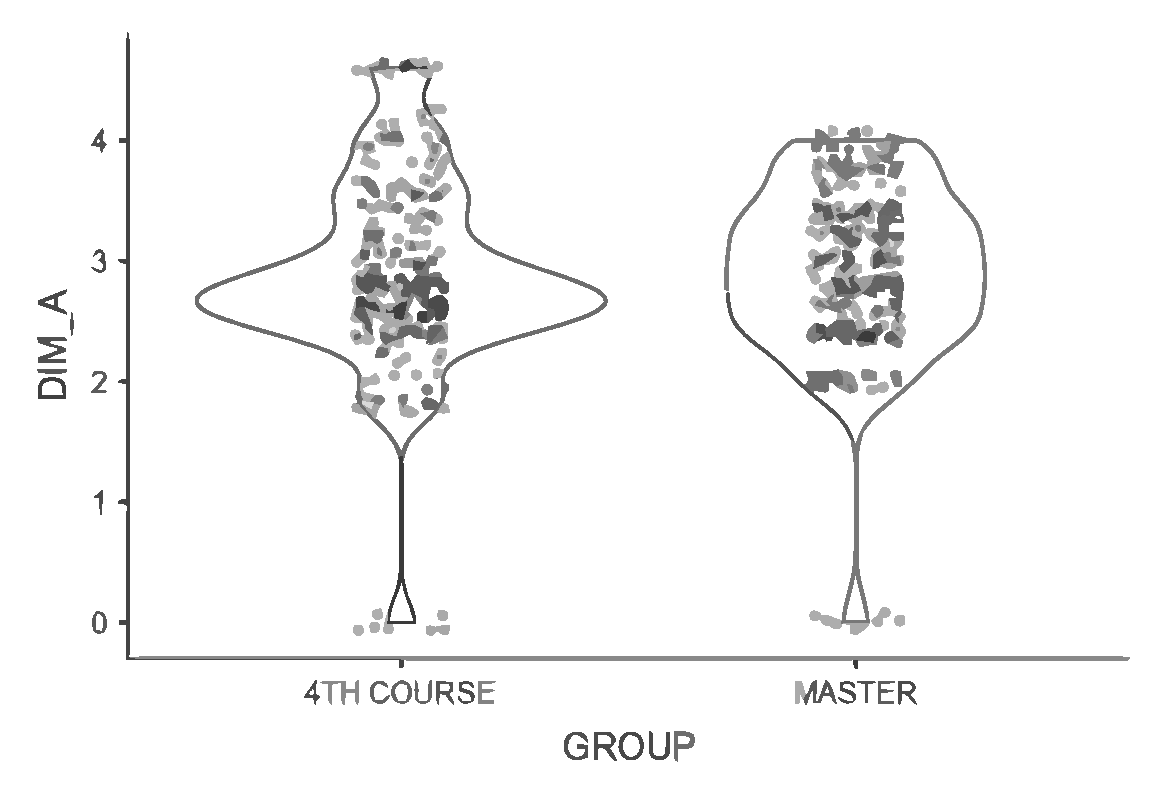
\includegraphics[width=\textwidth]{Figuras/fig1.png}
\caption{Etapas del desarrollo metodológico.}\label{fig-1}
\source{elaboración propia.}
\end{minipage}
\end{figure}


La descripción detallada de cada una de las etapas se presenta en la Tabla \ref{tab-1}.

%--- codigo da tabela 1 ---%
\begin{longtable}{p{0.28\textwidth} p{0.67\textwidth}}
\caption{Paso a paso de la metodología.}
\label{tab-1} \\
\toprule
Etapas & Descripción \\
\midrule
\endfirsthead

\endhead

Etapa 1: selección del tema de investigación &
El objetivo de esta investigación es examinar el avance de la computación en la nube en el proceso de adopción de tecnologías. Para ello, se han seleccionado como criterios de búsqueda los términos ``computación en la nube'' y ``adopción de tecnologías'', permitiendo un enfoque detallado en la evolución y el impacto de esta innovación. \\

Etapa 2: base de datos escogida. &
Según \textcite{ardanuy2012}, Elsevier introdujo Scopus como una base de datos con gran capacidad de publicación. A diferencia de Web of Science, Scopus se ha consolidado como una fuente destacada, indexando alrededor de 9.300 revistas de prestigio internacional. Su cobertura supera en un 66,07 \% a la de WoS y Dimensions \cite{singh2021}. \\

Etapa 3: ecuación y tesauros de búsqueda. &
``computación en la nube'' como: ``cloud computing'', ``cloud services'' y ``cloud'' y ``adopción de tecnologías'': ``technology adoption'', ``information technology adoption'' y ``adoption of information technology''. \\

& Ecuación de búsqueda: ( ( TITLE-ABS-KEY ( ``cloud computing'' ) OR TITLE-ABS-KEY ( cloud ) OR TITLE-ABS-KEY ( ``cloud service'' ) ) AND ( TITLE-ABS-KEY ( ``technology adoption'' ) OR TITLE-ABS-KEY ( ``information technology adoption'' ) OR TITLE-ABS-KEY ( ``adoption of information technology'' ) ) ) AND PUBYEAR > 2012 AND PUBYEAR < 2025 AND ( LIMIT-TO ( SUBJAREA , ``COMP'' ) OR LIMIT-TO ( SUBJAREA , ``BUSI'' ) OR LIMIT-TO ( SUBJAREA , ``ENGI'' ) OR LIMIT-TO ( SUBJAREA , ``SOCI'' ) ) AND ( LIMIT-TO ( DOCTYPE , ``ar'' ) ) AND ( LIMIT-TO ( LANGUAGE , ``English'' ) OR LIMIT-TO ( LANGUAGE , ``Spanish'' ) ).
\newline

Se obtuvieron 244 artículos completando todo el año 2024. \\

Etapa 4: software utilizado y depuración de la información. &
En la primera fase, los datos fueron depurados en Microsoft Excel. Luego, la información se transfirió a VOSviewer. \\

Etapa 5: análisis de los resultados. &
Se obtuvieron: los autores de mayor producción científica, la cantidad de documentos por año, las publicaciones por países, los artículos más citados y las revistas de mayor producción. \\

\bottomrule
\source{elaboración propia.}
\end{longtable}

Los criterios de inclusión y exclusión se observan en la Tabla \ref{fig-2}.

\begin{table}[h!]
  \centering
  \begin{threeparttable}
    \caption{Criterios de inclusión y exclusión.}
    \begin{tabular}{ll}
      \toprule
      Criterios de inclusión & Criterios de exclusión \\
      \midrule
      Publicaciones entre los años 2013 y 2024 & Publicaciones antes del año 2013 \\
      Idioma inglés y español & Diferentes al inglés y español \\
      Artículos indexados en Scopus & Artículos no indexadas en Scopus \\
      No capítulos de libros o conferencias & Capítulos de libros o conferencias \\
      \bottomrule
    \end{tabular}
\source{elaboración propia.}
  \end{threeparttable}
\end{table}

La selección detallada de la inclusión de los artículos se observa en la Figura \ref{fig-2}.

%--- codigo da figura 2 ---%
\begin{figure}[h!]
\centering
\begin{minipage}{.75\textwidth}
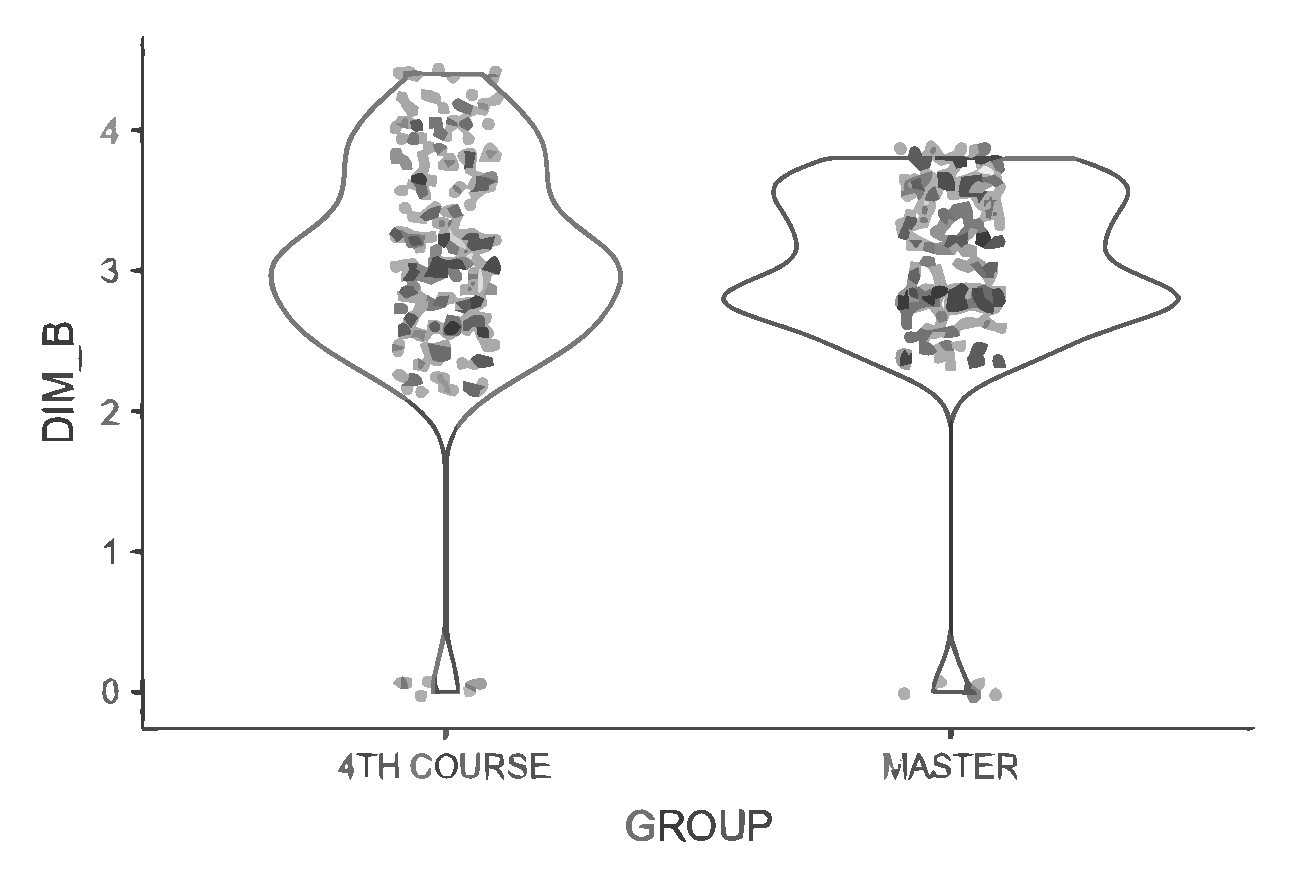
\includegraphics[width=\textwidth]{Figuras/fig2.png}
\caption{Diagrama de flujo de la selección de los estudios.}
\label{fig-2}
\source{elaboración propia.}
\end{minipage}
\end{figure}

\section{Resultados y discusión}\label{sec-results}
La adopción de computación en la nube varía significativamente entre países desarrollados y en desarrollo, influenciada por factores como infraestructura tecnológica, políticas gubernamentales y nivel de inversión e innovación. La Figura \ref{fig-3} compara seis países, tres de cada uno, para ilustrar estas diferencias. Su visualización permite identificar tendencias clave en el uso de servicios en la nube y su impacto en el desarrollo digital global.

%--- codigo da figura 3 ---%
\begin{figure}[h!]
\centering
\begin{minipage}{.75\textwidth}
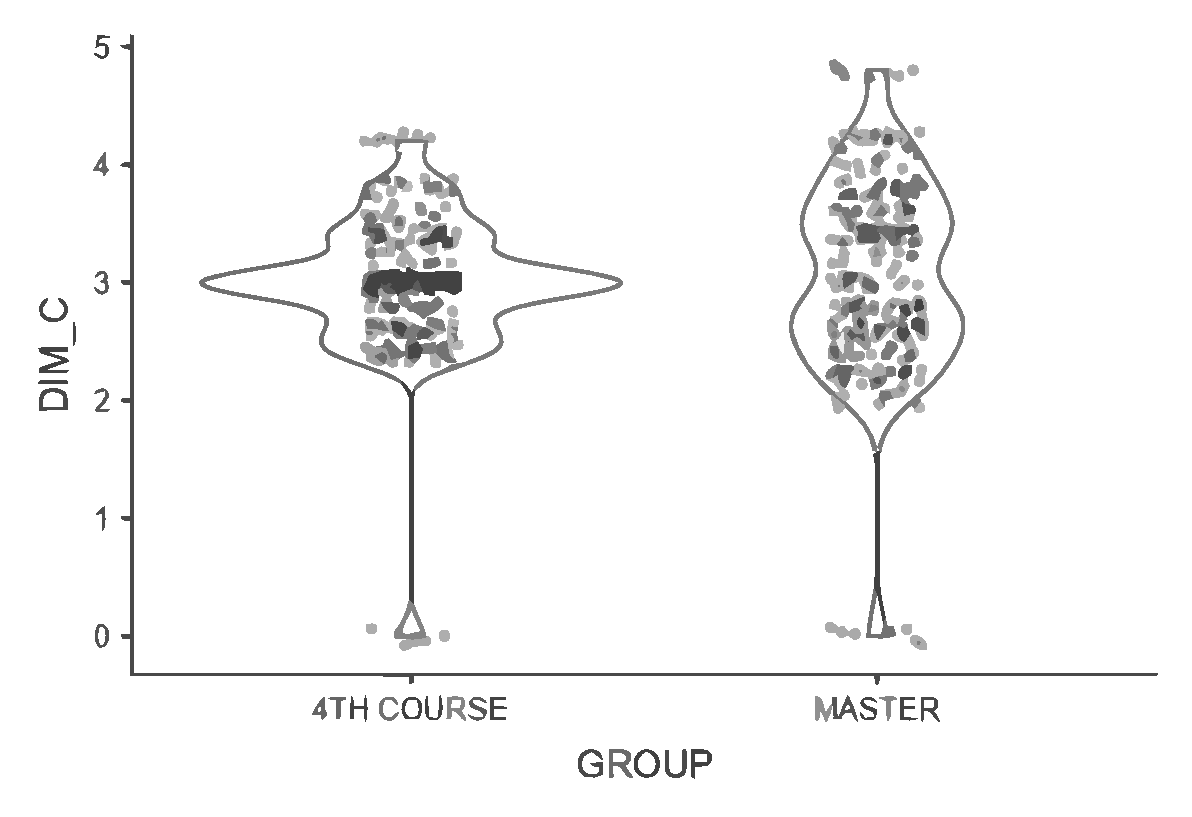
\includegraphics[width=\textwidth]{Figuras/fig3.png}
\caption{Comparación de la adopción de computación en la nube entre países desarrollados y países en desarrollo.}
\label{fig-3}
\source{elaboración propia a partir de: \textcite{cloudzero2025}; \textcite{nttdata2023} y \textcite{andi2023}.}
\end{minipage}
\end{figure}

\subsection{Análisis de desempeño}

\subsubsection{Producción científica}
Se analizó un periodo de 11 años a partir del 2013, con el objetivo de observar el avance del tema, teniendo en cuenta los textos publicados hasta el año 2024. En total se obtuvieron 244 artículos (Figura \ref{fig-4}). Las investigaciones halladas presentan un total de 6.759 citaciones. En los primeros años analizados, se observa una tendencia baja de artículos publicados (entre 4 y 5), desde el año 2015 hasta el año 2019 se evidencia un crecimiento entre 10 y 19 artículos, lo cual indica que es tema de interés por parte de la comunidad académica, puesto que a partir del año 2020 hubo un aumento del 70 \% en las publicaciones.

%--- codigo da figura 4 ---%
\begin{figure}[h!]
\centering
\begin{minipage}{.85\textwidth}
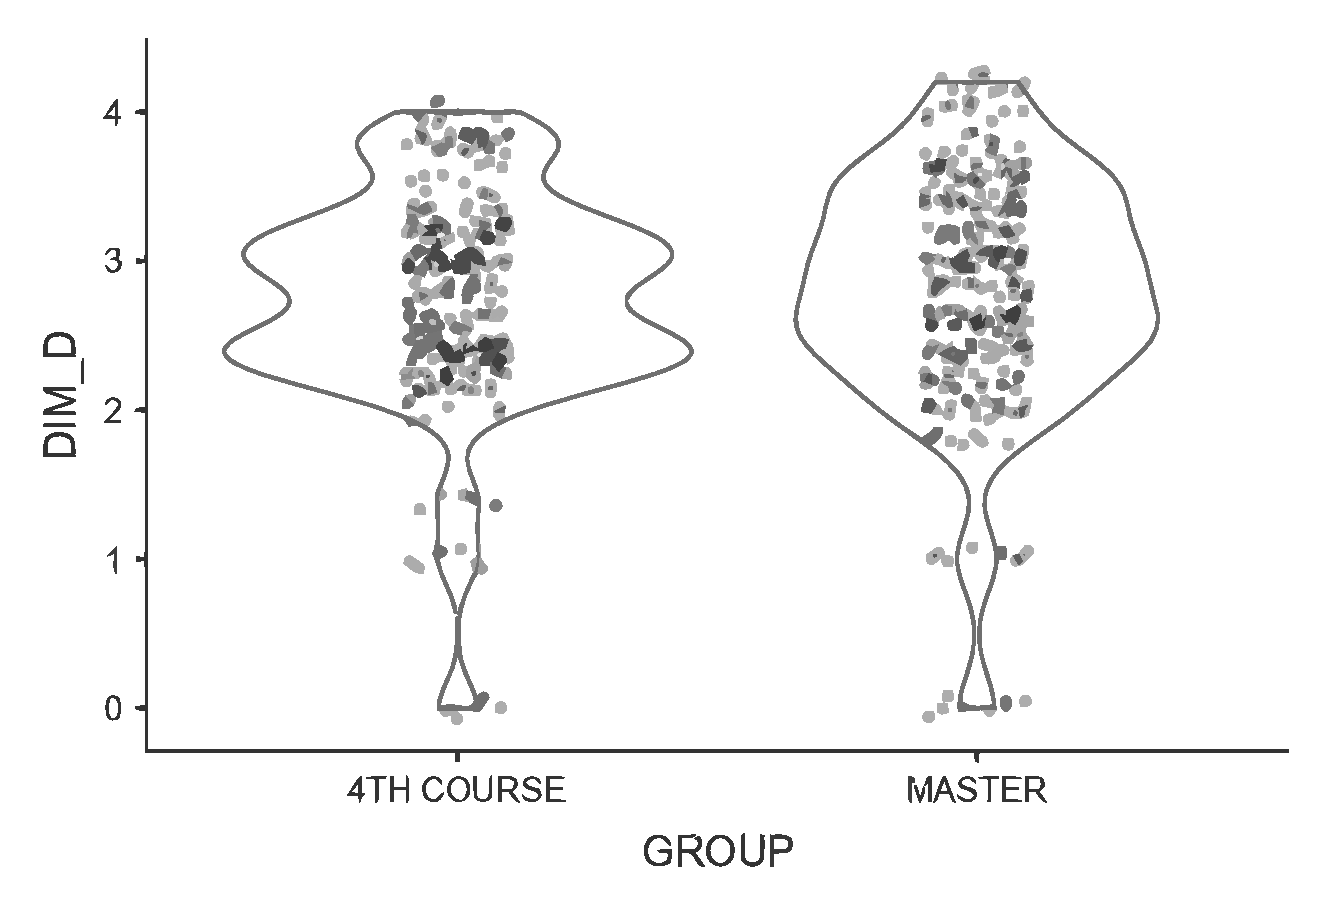
\includegraphics[width=\textwidth]{Figuras/fig4.png}
\caption{Evolución de la producción científica.}
\label{fig-4}
\source{elaboración propia.}
\end{minipage}
\end{figure}

Los estudios publicados en 2013 exploran distintos enfoques sobre la adopción de tecnologías emergentes. \textcite{khanagha2013} destacan la importancia de un proceso gradual para preservar activos organizacionales. \textcite{chen2013} analizan el impacto de los servicios bajo demanda en la estructura del mercado. En 2014, \textcite{subramanian2014}, mediante el modelo de difusión de la innovación (DOI), evidencian beneficios ecológicos y económicos de la nube. \textcite{demirkan2014} analizan sistemas de autoservicio en la nube que mejoran la eficiencia minorista, y \textcite{khan2014} propone un modelo que orienta a las organizaciones en su transición hacia tecnologías basadas en la nube. En 2015, varios estudios aportaron al análisis de la adopción de servicios en la nube desde diferentes enfoques. \textcite{salim2015} exploraron la relación entre la actitud del propietario y el control conductual percibido respecto a la intención de adopción, encontrando una asociación positiva con la actitud y negativa con el control percibido. El artículo más citado en este análisis es el de \textcite{parasuraman2015}, quienes desarrollaron el Índice de Preparación Tecnológica (TRI) y su versión TRI 2.0, aplicado al contexto del comercio móvil, redes sociales y computación en la nube. Este estudio validó la utilidad del TRI para segmentar usuarios según su disposición a adoptar tecnologías emergentes.

En 2016, diversos estudios ampliaron la comprensión de la adopción de la computación en la nube desde múltiples enfoques. \textcite{lansing2016} desarrollaron un modelo conceptual centrado en la confianza en los servicios en la nube, destacando su papel en la aceptación tecnológica. \textcite{mohammed2016} identificaron la fuerte influencia de factores organizacionales, tecnológicos y económicos en la adopción del gobierno electrónico basado en la nube. \textcite{sharma2016} propusieron un modelo híbrido para predecir la adopción entre profesionales de TI, encontrando que la confianza, la autoeficacia, la facilidad de uso y las oportunidades laborales son los principales motivadores. Para el año 2017, las investigaciones sobre computación en la nube se enfocaron en factores organizacionales y económicos. \textcite{obal2017} evidenció que presiones normativas y miméticas pueden disminuir la intención de adopción continua. \textcite{caldarelli2017} identificó la reducción de costos como un fuerte impulsor, mientras que \textcite{kumar2017}, a partir de una encuesta en PYMES indias, resaltó beneficios como ahorro, escalabilidad y acceso a tecnología actualizada. En 2018, el enfoque se amplió a aspectos psicológicos y sociales. \textcite{raut2018} aplicaron los modelos TOE, TAM y de riesgo, concluyendo que la confianza y el riesgo son barreras clave. \textcite{yim2018} destacaron la influencia de la propiedad psicológica en la percepción de utilidad.

En el 2019, las investigaciones se enfocaron en diversos factores que influyen en la adopción de la computación en la nube. \textcite{palossanchez2019} identificaron que el gobierno corporativo y las prácticas organizativas afectan significativamente la adopción tecnológica y el modelo de negocio. \textcite{dinca2019} destacaron que el conocimiento gerencial sobre la nube y los costos percibidos son los principales determinantes en su difusión. En 2020, se fortaleció el uso de marcos teóricos para comprender la adopción de la computación en la nube. \textcite{ahmed2020} aplicó el modelo TOE en pymes de Bangladesh, destacando la influencia de factores sociales, organizacionales y ambientales. \textcite{bhardwaj2020} integraron los modelos TAM, TOE y DOI en instituciones de educación superior en India, identificando elementos como apoyo institucional, compatibilidad y preparación tecnológica como facilitadores, mientras que la seguridad persistió como una barrera. En 2021, \textcite{matias2021} confirmaron que el apoyo regulatorio y la presión competitiva son factores decisivos en países en desarrollo. \textcite{mariani2021} encontraron, mediante el modelo TAM, que la confianza percibida mejora la utilidad y facilidad de uso, lo cual incrementa la intención de uso. En 2022, \textcite{ricobautista2022} ratificaron la aplicabilidad del TAM en universidades. \textcite{ilangakoon2022} demostraron que la adopción de tecnologías 4.0, incluida la nube, mejora el desempeño organizacional. \textcite{musyaffi2022} señalaron que variables como la calidad del sistema, el rol del instructor y la facilidad de uso percibida inciden directamente en la utilidad percibida, la intención de uso y la satisfacción del usuario en entornos educativos.

En 2023, diversos estudios coincidieron en destacar los beneficios de la integración de tecnologías de la industria 4.0. \textcite{battaglia2023}, \textcite{kavre2023} y \textcite{ling2023} demostraron que el desempeño organizacional mejora cuando estas tecnologías, incluida la computación en la nube, se fusionan de forma estratégica en lugar de implementarse de manera aislada. Por su parte, \textcite{qatawneh2024} analizó los factores que influyen en la adopción de la computación en la nube en el sector gubernamental de Jordania, destacando como claves el soporte de la alta dirección y el nivel de conocimiento en TI de los responsables de adopción. Por otro lado, \textcite{wang2024} estudiaron la transformación digital del sector bancario, enfocándose en tecnologías como la computación en la nube, big data e IA. Sus resultados evidenciaron la integración de sistemas heredados, el cumplimiento normativo y la gestión de riesgos de proveedores.

\subsubsection{Revistas más productivas}
240 revistas han publicado en el tema de computación en la nube y adopción de TI durante los últimos 10 años (2013 a 2024). Las 3 revistas más productivas corresponden a \textit{Technological Forecasting and Social Change}, \textit{Sustainability (Switzerland)} y \textit{Technology in Society}, con 12, 10 y 7 documentos, respectivamente, las cuales fueron citadas 748, 165 y 315 veces (Tabla \ref{tab-4}).

 %--- codigo da tabela 4 ---%
\begin{table}[h!]
  \centering
  \small
  \begin{threeparttable}
    \caption{Cinco revistas más productivas en el área de ``cloud computing'' y adopción de tecnologías.}\label{tab-4}
    \begin{tabular}{p{3cm}ccccr}
      \toprule
      Revista & Documentos & Número de citas & CiteScore SJR 2022 & Quartil SJR & Clúster \\
      \midrule
     \textit{Technological Forecasting and Social Change} & 16 & 1271 & 25,03 & Q1 & 1 \\
      \textit{Sustainability (Switzerland)} & 11 & 268 & 0,5153 & Q2 & 9 \\
      \textit{Technology in Society} & 8 & 556 & 11,239 & Q1 & 13 \\
      \textit{Journal of Enterprise Information Management} & 5 & 1236 & 19,227 & Q1 & 3 \\
      \textit{Computers in Human Behavior} & 4 & 448 & 19,422 & Q1 & 2 \\
      \bottomrule
    \end{tabular}
    \begin{tablenotes}
      \small
      \item \source{elaboración propia.}
    \end{tablenotes}
  \end{threeparttable}
\end{table}

\subsubsection{Contribuyentes clave}
Los 244 artículos analizados bajo el estudio bibliométrico corresponden a un total de 641 autores, de los cuales 27 contribuyeron con más de 2 artículos, es decir, el 11\% de los autores. Gardas, B. es el autor con mayor cantidad de artículos publicados en computación en la nube y adopción de TI (5 artículos); seguido por Priyadarshinee, P. con 4 documentos, y luego por los autores Ali, O., Khanagha, S., Raut, R., Sabi, H., Shrestha, A. y Uzoka, F., con 3 documentos publicados cada uno. El autor pionero en cuanto a mayor cantidad artículos publicados es Gardas, B., pues presenta 363 citas, una cifra que refleja la productividad y calidad. Por otro lado, Priyadarshinee, P. presenta 353 citas a partir de sus 4 artículos publicados, seguido por Ali, O., quien cuenta con 161 citas en sus 3 artículos (ver Figura \ref{fig-5}).

%--- codigo da figura 5 ---%
\begin{figure}[h!]
\centering
\begin{minipage}{.99\textwidth}
\includegraphics[width=\textwidth]{Figuras/fig5.png}
\caption{Autores pioneros.}
\label{fig-5}
\source{VOSviewer.}
\end{minipage}
\end{figure}

\subsubsection{Artículos más influyentes}
Se analizaron los artículos con mayor cantidad de citas, que corresponden a 33, todos con más de 80 citas y publicados entre los años 2013 y 2024, en la Tabla \ref{tab-5}, se muestran los cinco artículos con mayor cantidad de citas en el escalafón. El artículo con mayor cantidad de citas fue publicado en el año 2015, y acumula un total de 918 citas, los autores son: \textcite{parasuraman2015}. Los siguientes artículos con el mayor número de citas corresponden a \textcite{gangwar2015} y \textcite{barakabitze2020networkslicing}.


%--- codigo da tabela 5 ---%
\begin{longtable}{lp{1cm}p{4.5cm}p{3cm}r}
\caption{Cinco documentos más citados en el área.}
\label{tab-5}\\
\toprule
Autor(es) & Año & Documento & Journal & Citas \\
\midrule
\endfirsthead
\endhead

Parasuraman y Colby & 2015 & ``An Updated and Streamlined Technology Readiness Index: TRI 2.0'' & \textit{Journal of Service Research} & 918 \\

Gangwar \textit{et al.} & 2015 & ``Understanding determinants of cloud computing adoption using an integrated TAM-TOE model'' & \textit{Journal of Enterprise Information Management} & 774 \\

Barakabitze \textit{et al.} & 2020 & ``5G network slicing using SDN and NFV: A survey of taxonomy, architectures and future challenges'' & \textit{Computer Networks} & 607 \\

Javed \textit{et al.} & 2022 & ``Future smart cities requirements, emerging technologies, applications, challenges, and future aspects'' & \textit{Cities} & 381 \\

Saurabh y Dey & 2021 & ``Blockchain technology adoption, architecture, and sustainable agri-food supply chains'' & \textit{Journal of Cleaner Production} & 381 \\

\bottomrule
\source{elaboración propia basada en análisis de datos en Scopus.}
\end{longtable}


\subsection{Análisis de mapeo bibliométrico}

\subsubsection{Palabras clave}
En el análisis de coocurrencia de términos, el foco se dio en aquellos tesauros contenidos en el título, palabras clave y en el resumen de cada artículo. En este trabajo, se utilizó un mínimo de ocurrencia de 3. Gracias a este filtro, se obtuvo un total de 95 términos, que luego fueron depurados eliminando palabras en el contexto de cualquier investigación, como ``artículo'' e ``integración''. Otra depuración se hizo reemplazando las palabras que fueron sinónimos de otras. Este proceso dio como resultado un total de 83 palabras, asociadas a 15 grupos, en la Tabla \ref{tab-6} se muestran los 5 primeros clústeres.

%--- codigo da tabela 6 ---%
\begin{table}[htbp]
  \centering
  \begin{threeparttable}
    \caption{Clasificación de palabras clave.}\label{tab-6}
    \begin{tabular}{lp{12cm}}
      \toprule
      Clúster & Palabras clave \\
      \midrule
      Clúster 1 & Competencias digitales, tecnologías educativas, ambiente, adopción de tecnologías verdes, cuidado de la salud, teoría institucional, privacidad, SaaS, confianza, universidades, UTAUT2. \\
      Clúster 2 & Librerías académicas, IA, automatización, aprendizaje profundo, IOT, TI, nube móvil, seguridad de riesgo percibida, robots, TPB, UTAUT. \\
      Clúster 3 & Banco, construcción 4.0, tecnologías emergentes, finanzas, cuarta revolución industrial, hardware, innovación, aceptación tecnológica. \\
      Clúster 4 & Desarrollo económico, gobierno electrónico, educación superior, intención de adopción, SEM, efecto de las redes sociales. \\
      Clúster 5 & Analítica, beneficios, costos de los servicios, soporte a la toma de decisiones, generación de decisiones, oportunidades, riesgos. \\
      \bottomrule
    \end{tabular}
\source{elaboración propia análisis de VOSviewer.}
  \end{threeparttable}
\end{table}

Dentro del clúster 1 (rojo), donde aparece el término con mayor número de ocurrencias (adopción de tecnologías), aparecen otros términos, como el IoT y se caracteriza por artículos que se centran en estudiar la industria en la construcción, el comercio electrónico y la educación en ingeniería. El clúster 2 (verde) contiene el término TIC y tecnologías digitales, que se combinan con términos como la cadena de suministro y diversas variables como la ventaja competitiva y la creación de valor. Por otra parte, el clúster 3 (azul) se caracteriza por palabras que tienen que ver con la técnica de ecuaciones estructurales (SEM) teniendo en cuenta evaluaciones de riesgo, seguridad de los datos y desempeño industrial. En el clúster 4 (amarillo) se tiene la combinación de países desarrollados con el tema de privacidad y análisis de la información. El clúster 5 (morado) contiene el término con la segunda cantidad de ocurrencias más alta, es decir la computación en la nube, donde se combinan estudios empíricos y el tema de la confianza (ver Figura \ref{fig-6}).

%--- codigo da figura 6 ---%
\begin{figure}[h!]
\centering
\begin{minipage}{.99\textwidth}
\includegraphics[width=\textwidth]{Figuras/fig6.png}
\caption{Clústeres de palabras clave.}
\label{fig-6}
\source{VOSviewer.}
\end{minipage}
\end{figure}



\section{Conclusiones y discusión}\label{sec-conclusiones}
Aunque la literatura científica sobre computación en la nube ha mostrado un crecimiento constante, su adopción práctica varía significativamente entre regiones. Según \textcite{marston2011}, factores como la infraestructura tecnológica, seguridad y preparación organizacional determinan la implementación, siendo más favorables en países desarrollados que en aquellos en desarrollo, donde aún existen barreras estructurales. \textcite{ren2025} señalan la escasez de publicaciones recientes sobre el tema en Scopus y destacan a China, India y EE. UU. como los principales países productores. A través de un estudio bibliométrico basado en datos de Scopus y analizados con VOSviewer, se evidenció un crecimiento sostenido en la producción científica, con la participación de 756 autores, 74 países y 172 revistas, destacando el liderazgo de países desarrollados como EE. UU., China y Australia.

Los autores presentados en este estudio apuntan a las investigaciones en Bangladesh, España, Rumania, Taiwán y Portugal, entre otros. Diferentes autores se han preocupado por investigar los antecedentes de la adopción de diferentes TI, especialmente la computación en la nube, y han encontrado que la eficiencia \cite{obal2017}, la utilidad y facilidad de uso percibida \cite{narwane2019, yim2018, shetty2023, sharma2023}, la actitud \cite{mariani2021, salim2015}, la confianza \cite{chou2017, lansing2016, narwane2019, priyadarshinee2017, dajani2022}, el gobierno corporativo y los procedimientos y prácticas de la organización \cite{palossanchez2019}, los conocimientos de los administradores y los costos percibidos \cite{caldarelli2017, chou2017, dinca2019, doherty2015, pfister2023}, la compatibilidad \cite{chou2017}, la presión competitiva \cite{matias2021}, los elementos del marco TOE \cite{asiaei2019, safari2015}, las presiones miméticas y coercitivas \cite{yigitbasioglu2015}, la influencia social \cite{narwane2019}, y el riesgo de seguridad \cite{narwane2019, priyadarshinee2017, saura2023, mariani2021} son factores impulsores clave.

El autor que tiene mayor producción en el tema es Gardas, las revistas con mayores publicaciones son: \textit{Technological Forecasting and Social Change} y \textit{Sustainability (Switzerland)} categorizadas como Q1 y Q2 respectivamente, son relevantes en el ámbito de las aplicaciones tecnológicas en la educación, además sirven como plataformas de gran impacto para la difusión de investigaciones sobre tecnología en la educación. Los países más productivos son Malasia, Estados Unidos e India. En cuanto a número de colaboraciones, Estados Unidos colabora con 30 países, Malasia con 31 y China con 28. Estos resultados resaltan la alta cooperación internacional en este campo.  Los contribuyentes que más influyen de acuerdo con el número de citas, por autor: Date, Gangwar y Ramaswamy, por país: Estados Unidos, y por revista: \textit{Journal of Enterprise Information Management}. Además, el artículo más influyente de acuerdo con este calificativo es ``An Updated and Streamlined Technology Readiness Index: TRI 2.0'' por \textcite{parasuraman2015}.

Entre los temas más relevantes encontrados se destacan: tecnologías educativas, privacidad, confianza, automatización, aprendizaje profundo, internet de las cosas, robótica, industria 4.0, innovación y aceptación tecnológica, junto con marcos teóricos como la teoría institucional, la teoría del comportamiento planificado y la UTAUT2. El estudio aporta a la academia al facilitar el acceso al conocimiento científico, fomentar redes de colaboración entre investigadores, e identificar áreas clave para quienes comienzan a investigar en este campo emergente.

\section{Limitaciones y futuras líneas de investigación}
Esta investigación presenta algunas limitaciones, entre ellas, el uso exclusivo del software libre VOSviewer, que solo permite el análisis de una base de datos a la vez, en este caso Scopus, lo cual excluye otras fuentes relevantes como Web of Science, Dimensions o Google Scholar. Además, se restringió el análisis a artículos en idioma inglés y español, lo que podría limitar la diversidad del conocimiento incluido. Durante el estudio, se identificaron diversos vacíos en la literatura, sintetizados en la Figura \ref{fig-7} y extraídos de los artículos revisados. De manera cronológica, se destacan propuestas como: estudiar el impacto de la seguridad y el apoyo directivo \cite{subramanian2014}; incluir a los no adoptantes en investigaciones futuras \cite{gangwar2015}; aplicar el marco TOE a nivel individual y explorar sectores no empresariales \cite{safari2015, shetty2023}; analizar factores de adopción con teorías como TAM \cite{hidayanto2015, ho2017trust} y UTAUT \cite{hidayanto2015, ali2019}; así como examinar la transición de la intención al comportamiento real de uso \cite{salim2015}.

Entre los años 2016 y 2021, diversos estudios sugieren futuras líneas de investigación relacionadas con la adopción de la computación en la nube. En 2016, se propone ampliar los modelos tradicionales de adopción incluyendo variables como la oportunidad laboral \cite{sharma2016} y factores socioculturales \cite{sabi2016}. Durante 2017, se destacan la aceptación de herramientas específicas como Dropbox y Google Docs en el ámbito educativo \cite{shana_abulibdeh2017cloud}, y la necesidad de abordar de forma diferenciada los modelos LaaS, PaaS y SaaS \cite{arvanitis2017cloud, chen_chen_lee2018sustainability}. En 2018, se recomienda investigar el impacto del uso de la nube en el desempeño organizacional \cite{raut2018, saura2023}. Para el año 2020, \textcite{bongo2020industry4} proponen explorar la autorregulación individual como análisis relevante para comprender la adopción. En 2021, \textcite{mariani2021} sugieren profundizar en las condiciones contextuales bajo las cuales el riesgo percibido y las brechas de seguridad influyen en la adopción sostenida. \textcite{andrews2021} plantean incluir características individuales en la decisión de adoptar tecnologías. Finalmente, \textcite{zulherman2021} enfatizan en investigar la adopción de tecnologías en línea específicamente en contextos educativos.

En el año 2022, \textcite{musyaffi2022} destacan la importancia de centrarse en la satisfacción del estudiante al utilizar medios de aprendizaje para aumentar el rendimiento académico. Otro aspecto importante es estudiar diferentes variables mediadas por aspectos como la confianza percibida, la satisfacción del usuario o los valores culturales \cite{dajani2022}. Finalmente, en el año 2023, \textcite{saura2023} sugieren estudiar el efecto de la adopción de las TI en cuanto a crecimiento empresarial y creación de valor. Por su lado, \textcite{rehman2023} proponen explorar otras innovaciones tecnológicas (e.g. IA) potenciales que puedan impactar el financiamiento de las PYMES (ver Figura \ref{fig-7}).

%--- codigo da figura 7 ---%
\begin{figure}[h!]
\centering
\begin{minipage}{.99\textwidth}
\includegraphics[width=\textwidth]{Figuras/fig7.png}
\caption{Futuras líneas de investigación.}
\label{fig-7}
\source{elaboración propia.}
\end{minipage}
\end{figure}

\newpage
\printbibliography\label{sec-bib}
% if the text is not in Portuguese, it might be necessary to use the code below instead to print the correct ABNT abbreviations [s.n.], [s.l.]
%\begin{portuguese}
%\printbibliography[title={Bibliography}]
%\end{portuguese}


%full list: conceptualization,datacuration,formalanalysis,funding,investigation,methodology,projadm,resources,software,supervision,validation,visualization,writing,review
\begin{contributors}[sec-contributors]
\authorcontribution{Leidy Johanna Botero Toro}[investigation,datacuration,formalanalysis,writing]
\authorcontribution{Miguel Solís-Molina}[review]
\authorcontribution{Augusto Rodriguez-Orejuela}[supervision]
\end{contributors}

\begin{dataavailability}
\txtdataavailability{databody} % options: dataavailable, dataonly, databody, datanotav, nodata
\end{dataavailability}


\end{document}

